\begin{figure}[htbp]\centering
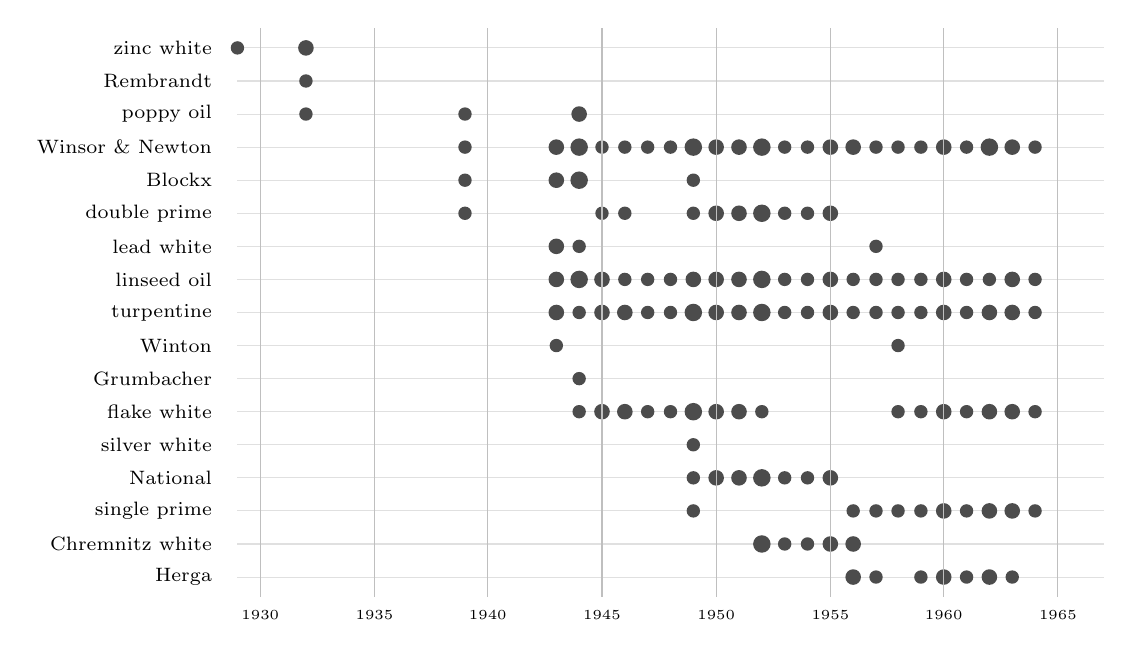
\begin{tikzpicture}
\node[anchor=east,font=\scriptsize] at (-0.2,0.00) {zinc white};
\draw[black!12] (0,0.00) -- (11,0.00);
\fill[black!70] (0.00,0.00) circle (0.085);
\fill[black!70] (0.87,0.00) circle (0.099);
\node[anchor=east,font=\scriptsize] at (-0.2,-0.42) {Rembrandt};
\draw[black!12] (0,-0.42) -- (11,-0.42);
\fill[black!70] (0.87,-0.42) circle (0.085);
\node[anchor=east,font=\scriptsize] at (-0.2,-0.84) {poppy oil};
\draw[black!12] (0,-0.84) -- (11,-0.84);
\fill[black!70] (0.87,-0.84) circle (0.085);
\fill[black!70] (2.89,-0.84) circle (0.085);
\fill[black!70] (4.34,-0.84) circle (0.099);
\node[anchor=east,font=\scriptsize] at (-0.2,-1.26) {Winsor \& Newton};
\draw[black!12] (0,-1.26) -- (11,-1.26);
\fill[black!70] (2.89,-1.26) circle (0.085);
\fill[black!70] (4.05,-1.26) circle (0.099);
\fill[black!70] (4.34,-1.26) circle (0.111);
\fill[black!70] (4.63,-1.26) circle (0.085);
\fill[black!70] (4.92,-1.26) circle (0.085);
\fill[black!70] (5.21,-1.26) circle (0.085);
\fill[black!70] (5.50,-1.26) circle (0.085);
\fill[black!70] (5.79,-1.26) circle (0.111);
\fill[black!70] (6.08,-1.26) circle (0.099);
\fill[black!70] (6.37,-1.26) circle (0.099);
\fill[black!70] (6.66,-1.26) circle (0.111);
\fill[black!70] (6.95,-1.26) circle (0.085);
\fill[black!70] (7.24,-1.26) circle (0.085);
\fill[black!70] (7.53,-1.26) circle (0.099);
\fill[black!70] (7.82,-1.26) circle (0.099);
\fill[black!70] (8.11,-1.26) circle (0.085);
\fill[black!70] (8.39,-1.26) circle (0.085);
\fill[black!70] (8.68,-1.26) circle (0.085);
\fill[black!70] (8.97,-1.26) circle (0.099);
\fill[black!70] (9.26,-1.26) circle (0.085);
\fill[black!70] (9.55,-1.26) circle (0.111);
\fill[black!70] (9.84,-1.26) circle (0.099);
\fill[black!70] (10.13,-1.26) circle (0.085);
\node[anchor=east,font=\scriptsize] at (-0.2,-1.68) {Blockx};
\draw[black!12] (0,-1.68) -- (11,-1.68);
\fill[black!70] (2.89,-1.68) circle (0.085);
\fill[black!70] (4.05,-1.68) circle (0.099);
\fill[black!70] (4.34,-1.68) circle (0.111);
\fill[black!70] (5.79,-1.68) circle (0.085);
\node[anchor=east,font=\scriptsize] at (-0.2,-2.10) {double prime};
\draw[black!12] (0,-2.10) -- (11,-2.10);
\fill[black!70] (2.89,-2.10) circle (0.085);
\fill[black!70] (4.63,-2.10) circle (0.085);
\fill[black!70] (4.92,-2.10) circle (0.085);
\fill[black!70] (5.79,-2.10) circle (0.085);
\fill[black!70] (6.08,-2.10) circle (0.099);
\fill[black!70] (6.37,-2.10) circle (0.099);
\fill[black!70] (6.66,-2.10) circle (0.111);
\fill[black!70] (6.95,-2.10) circle (0.085);
\fill[black!70] (7.24,-2.10) circle (0.085);
\fill[black!70] (7.53,-2.10) circle (0.099);
\node[anchor=east,font=\scriptsize] at (-0.2,-2.52) {lead white};
\draw[black!12] (0,-2.52) -- (11,-2.52);
\fill[black!70] (4.05,-2.52) circle (0.099);
\fill[black!70] (4.34,-2.52) circle (0.085);
\fill[black!70] (8.11,-2.52) circle (0.085);
\node[anchor=east,font=\scriptsize] at (-0.2,-2.94) {linseed oil};
\draw[black!12] (0,-2.94) -- (11,-2.94);
\fill[black!70] (4.05,-2.94) circle (0.099);
\fill[black!70] (4.34,-2.94) circle (0.111);
\fill[black!70] (4.63,-2.94) circle (0.099);
\fill[black!70] (4.92,-2.94) circle (0.085);
\fill[black!70] (5.21,-2.94) circle (0.085);
\fill[black!70] (5.50,-2.94) circle (0.085);
\fill[black!70] (5.79,-2.94) circle (0.099);
\fill[black!70] (6.08,-2.94) circle (0.099);
\fill[black!70] (6.37,-2.94) circle (0.099);
\fill[black!70] (6.66,-2.94) circle (0.111);
\fill[black!70] (6.95,-2.94) circle (0.085);
\fill[black!70] (7.24,-2.94) circle (0.085);
\fill[black!70] (7.53,-2.94) circle (0.099);
\fill[black!70] (7.82,-2.94) circle (0.085);
\fill[black!70] (8.11,-2.94) circle (0.085);
\fill[black!70] (8.39,-2.94) circle (0.085);
\fill[black!70] (8.68,-2.94) circle (0.085);
\fill[black!70] (8.97,-2.94) circle (0.099);
\fill[black!70] (9.26,-2.94) circle (0.085);
\fill[black!70] (9.55,-2.94) circle (0.085);
\fill[black!70] (9.84,-2.94) circle (0.099);
\fill[black!70] (10.13,-2.94) circle (0.085);
\node[anchor=east,font=\scriptsize] at (-0.2,-3.36) {turpentine};
\draw[black!12] (0,-3.36) -- (11,-3.36);
\fill[black!70] (4.05,-3.36) circle (0.099);
\fill[black!70] (4.34,-3.36) circle (0.085);
\fill[black!70] (4.63,-3.36) circle (0.099);
\fill[black!70] (4.92,-3.36) circle (0.099);
\fill[black!70] (5.21,-3.36) circle (0.085);
\fill[black!70] (5.50,-3.36) circle (0.085);
\fill[black!70] (5.79,-3.36) circle (0.111);
\fill[black!70] (6.08,-3.36) circle (0.099);
\fill[black!70] (6.37,-3.36) circle (0.099);
\fill[black!70] (6.66,-3.36) circle (0.111);
\fill[black!70] (6.95,-3.36) circle (0.085);
\fill[black!70] (7.24,-3.36) circle (0.085);
\fill[black!70] (7.53,-3.36) circle (0.099);
\fill[black!70] (7.82,-3.36) circle (0.085);
\fill[black!70] (8.11,-3.36) circle (0.085);
\fill[black!70] (8.39,-3.36) circle (0.085);
\fill[black!70] (8.68,-3.36) circle (0.085);
\fill[black!70] (8.97,-3.36) circle (0.099);
\fill[black!70] (9.26,-3.36) circle (0.085);
\fill[black!70] (9.55,-3.36) circle (0.099);
\fill[black!70] (9.84,-3.36) circle (0.099);
\fill[black!70] (10.13,-3.36) circle (0.085);
\node[anchor=east,font=\scriptsize] at (-0.2,-3.78) {Winton};
\draw[black!12] (0,-3.78) -- (11,-3.78);
\fill[black!70] (4.05,-3.78) circle (0.085);
\fill[black!70] (8.39,-3.78) circle (0.085);
\node[anchor=east,font=\scriptsize] at (-0.2,-4.20) {Grumbacher};
\draw[black!12] (0,-4.20) -- (11,-4.20);
\fill[black!70] (4.34,-4.20) circle (0.085);
\node[anchor=east,font=\scriptsize] at (-0.2,-4.62) {flake white};
\draw[black!12] (0,-4.62) -- (11,-4.62);
\fill[black!70] (4.34,-4.62) circle (0.085);
\fill[black!70] (4.63,-4.62) circle (0.099);
\fill[black!70] (4.92,-4.62) circle (0.099);
\fill[black!70] (5.21,-4.62) circle (0.085);
\fill[black!70] (5.50,-4.62) circle (0.085);
\fill[black!70] (5.79,-4.62) circle (0.111);
\fill[black!70] (6.08,-4.62) circle (0.099);
\fill[black!70] (6.37,-4.62) circle (0.099);
\fill[black!70] (6.66,-4.62) circle (0.085);
\fill[black!70] (8.39,-4.62) circle (0.085);
\fill[black!70] (8.68,-4.62) circle (0.085);
\fill[black!70] (8.97,-4.62) circle (0.099);
\fill[black!70] (9.26,-4.62) circle (0.085);
\fill[black!70] (9.55,-4.62) circle (0.099);
\fill[black!70] (9.84,-4.62) circle (0.099);
\fill[black!70] (10.13,-4.62) circle (0.085);
\node[anchor=east,font=\scriptsize] at (-0.2,-5.04) {silver white};
\draw[black!12] (0,-5.04) -- (11,-5.04);
\fill[black!70] (5.79,-5.04) circle (0.085);
\node[anchor=east,font=\scriptsize] at (-0.2,-5.46) {National};
\draw[black!12] (0,-5.46) -- (11,-5.46);
\fill[black!70] (5.79,-5.46) circle (0.085);
\fill[black!70] (6.08,-5.46) circle (0.099);
\fill[black!70] (6.37,-5.46) circle (0.099);
\fill[black!70] (6.66,-5.46) circle (0.111);
\fill[black!70] (6.95,-5.46) circle (0.085);
\fill[black!70] (7.24,-5.46) circle (0.085);
\fill[black!70] (7.53,-5.46) circle (0.099);
\node[anchor=east,font=\scriptsize] at (-0.2,-5.88) {single prime};
\draw[black!12] (0,-5.88) -- (11,-5.88);
\fill[black!70] (5.79,-5.88) circle (0.085);
\fill[black!70] (7.82,-5.88) circle (0.085);
\fill[black!70] (8.11,-5.88) circle (0.085);
\fill[black!70] (8.39,-5.88) circle (0.085);
\fill[black!70] (8.68,-5.88) circle (0.085);
\fill[black!70] (8.97,-5.88) circle (0.099);
\fill[black!70] (9.26,-5.88) circle (0.085);
\fill[black!70] (9.55,-5.88) circle (0.099);
\fill[black!70] (9.84,-5.88) circle (0.099);
\fill[black!70] (10.13,-5.88) circle (0.085);
\node[anchor=east,font=\scriptsize] at (-0.2,-6.30) {Chremnitz white};
\draw[black!12] (0,-6.30) -- (11,-6.30);
\fill[black!70] (6.66,-6.30) circle (0.111);
\fill[black!70] (6.95,-6.30) circle (0.085);
\fill[black!70] (7.24,-6.30) circle (0.085);
\fill[black!70] (7.53,-6.30) circle (0.099);
\fill[black!70] (7.82,-6.30) circle (0.099);
\node[anchor=east,font=\scriptsize] at (-0.2,-6.72) {Herga};
\draw[black!12] (0,-6.72) -- (11,-6.72);
\fill[black!70] (7.82,-6.72) circle (0.099);
\fill[black!70] (8.11,-6.72) circle (0.085);
\fill[black!70] (8.68,-6.72) circle (0.085);
\fill[black!70] (8.97,-6.72) circle (0.099);
\fill[black!70] (9.26,-6.72) circle (0.085);
\fill[black!70] (9.55,-6.72) circle (0.099);
\fill[black!70] (9.84,-6.72) circle (0.085);
\draw[black!25] (0.29,0.25) -- (0.29,-6.97); \node[font=\tiny,anchor=north] at (0.29,-7.02) {1930};
\draw[black!25] (1.74,0.25) -- (1.74,-6.97); \node[font=\tiny,anchor=north] at (1.74,-7.02) {1935};
\draw[black!25] (3.18,0.25) -- (3.18,-6.97); \node[font=\tiny,anchor=north] at (3.18,-7.02) {1940};
\draw[black!25] (4.63,0.25) -- (4.63,-6.97); \node[font=\tiny,anchor=north] at (4.63,-7.02) {1945};
\draw[black!25] (6.08,0.25) -- (6.08,-6.97); \node[font=\tiny,anchor=north] at (6.08,-7.02) {1950};
\draw[black!25] (7.53,0.25) -- (7.53,-6.97); \node[font=\tiny,anchor=north] at (7.53,-7.02) {1955};
\draw[black!25] (8.97,0.25) -- (8.97,-6.97); \node[font=\tiny,anchor=north] at (8.97,-7.02) {1960};
\draw[black!25] (10.42,0.25) -- (10.42,-6.97); \node[font=\tiny,anchor=north] at (10.42,-7.02) {1965};
\end{tikzpicture}
\caption{A succession, not a preference: each material against the years the leaves date it to, earliest first, one dot to a year and its size standing for how many works that year names it. Rembrandt colours and zinc white in poppy oil at the start; Winsor \& Newton and flake white in linseed oil and turpentine from the middle 1940s; the canvas turning from National to Herga and the priming from double to single across the 1950s. Only the 43 works dated by the leaf itself are plotted. After the Technique tab. Drawn by Claude Fable~5.1, from \texttt{materials.json} (undated).}\label{fig:materials}
\end{figure}
